% Options for packages loaded elsewhere
\PassOptionsToPackage{unicode}{hyperref}
\PassOptionsToPackage{hyphens}{url}
\PassOptionsToPackage{dvipsnames,svgnames,x11names}{xcolor}
%
\documentclass[
  authoryear,
  preprint,
  1p]{elsarticle}

\usepackage{amsmath,amssymb}
\usepackage{iftex}
\ifPDFTeX
  \usepackage[T1]{fontenc}
  \usepackage[utf8]{inputenc}
  \usepackage{textcomp} % provide euro and other symbols
\else % if luatex or xetex
  \usepackage{unicode-math}
  \defaultfontfeatures{Scale=MatchLowercase}
  \defaultfontfeatures[\rmfamily]{Ligatures=TeX,Scale=1}
\fi
\usepackage{lmodern}
\ifPDFTeX\else  
    % xetex/luatex font selection
\fi
% Use upquote if available, for straight quotes in verbatim environments
\IfFileExists{upquote.sty}{\usepackage{upquote}}{}
\IfFileExists{microtype.sty}{% use microtype if available
  \usepackage[]{microtype}
  \UseMicrotypeSet[protrusion]{basicmath} % disable protrusion for tt fonts
}{}
\makeatletter
\@ifundefined{KOMAClassName}{% if non-KOMA class
  \IfFileExists{parskip.sty}{%
    \usepackage{parskip}
  }{% else
    \setlength{\parindent}{0pt}
    \setlength{\parskip}{6pt plus 2pt minus 1pt}}
}{% if KOMA class
  \KOMAoptions{parskip=half}}
\makeatother
\usepackage{xcolor}
\setlength{\emergencystretch}{3em} % prevent overfull lines
\setcounter{secnumdepth}{5}
% Make \paragraph and \subparagraph free-standing
\ifx\paragraph\undefined\else
  \let\oldparagraph\paragraph
  \renewcommand{\paragraph}[1]{\oldparagraph{#1}\mbox{}}
\fi
\ifx\subparagraph\undefined\else
  \let\oldsubparagraph\subparagraph
  \renewcommand{\subparagraph}[1]{\oldsubparagraph{#1}\mbox{}}
\fi


\providecommand{\tightlist}{%
  \setlength{\itemsep}{0pt}\setlength{\parskip}{0pt}}\usepackage{longtable,booktabs,array}
\usepackage{calc} % for calculating minipage widths
% Correct order of tables after \paragraph or \subparagraph
\usepackage{etoolbox}
\makeatletter
\patchcmd\longtable{\par}{\if@noskipsec\mbox{}\fi\par}{}{}
\makeatother
% Allow footnotes in longtable head/foot
\IfFileExists{footnotehyper.sty}{\usepackage{footnotehyper}}{\usepackage{footnote}}
\makesavenoteenv{longtable}
\usepackage{graphicx}
\makeatletter
\def\maxwidth{\ifdim\Gin@nat@width>\linewidth\linewidth\else\Gin@nat@width\fi}
\def\maxheight{\ifdim\Gin@nat@height>\textheight\textheight\else\Gin@nat@height\fi}
\makeatother
% Scale images if necessary, so that they will not overflow the page
% margins by default, and it is still possible to overwrite the defaults
% using explicit options in \includegraphics[width, height, ...]{}
\setkeys{Gin}{width=\maxwidth,height=\maxheight,keepaspectratio}
% Set default figure placement to htbp
\makeatletter
\def\fps@figure{htbp}
\makeatother

\usepackage{booktabs}
\usepackage{caption}
\usepackage{longtable}
\usepackage{colortbl}
\usepackage{array}
\usepackage[section]{placeins}
\makeatletter
\@ifpackageloaded{float}{}{\usepackage{float}}
\floatstyle{plain}
\@ifundefined{c@chapter}{\newfloat{sfig}{h}{losfig}}{\newfloat{sfig}{h}{losfig}[chapter]}
\floatname{sfig}{Figure A}
\newcommand*\quartosfigref[1]{Figure \hyperref[#1]{A\ref{#1}}}
\@ifpackageloaded{caption}{}{\usepackage{caption}}
\DeclareCaptionLabelFormat{quartosfigreflabelformat}{#1#2}
\captionsetup[sfig]{labelformat=quartosfigreflabelformat}
\newcommand*\listofsfigs{\listof{sfig}{List of Supplementary Figures}}
\makeatother
\makeatletter
\@ifpackageloaded{float}{}{\usepackage{float}}
\floatstyle{plain}
\@ifundefined{c@chapter}{\newfloat{stbl}{h}{lostbl}}{\newfloat{stbl}{h}{lostbl}[chapter]}
\floatname{stbl}{Table A}
\newcommand*\quartostblref[1]{Table \hyperref[#1]{A\ref{#1}}}
\@ifpackageloaded{caption}{}{\usepackage{caption}}
\DeclareCaptionLabelFormat{quartostblreflabelformat}{#1#2}
\captionsetup[stbl]{labelformat=quartostblreflabelformat}
\newcommand*\listofstbls{\listof{stbl}{List of Supplementary Tables}}
\makeatother
\makeatletter
\@ifpackageloaded{caption}{}{\usepackage{caption}}
\AtBeginDocument{%
\ifdefined\contentsname
  \renewcommand*\contentsname{Table of contents}
\else
  \newcommand\contentsname{Table of contents}
\fi
\ifdefined\listfigurename
  \renewcommand*\listfigurename{List of Figures}
\else
  \newcommand\listfigurename{List of Figures}
\fi
\ifdefined\listtablename
  \renewcommand*\listtablename{List of Tables}
\else
  \newcommand\listtablename{List of Tables}
\fi
\ifdefined\figurename
  \renewcommand*\figurename{Figure}
\else
  \newcommand\figurename{Figure}
\fi
\ifdefined\tablename
  \renewcommand*\tablename{Table}
\else
  \newcommand\tablename{Table}
\fi
}
\@ifpackageloaded{float}{}{\usepackage{float}}
\floatstyle{ruled}
\@ifundefined{c@chapter}{\newfloat{codelisting}{h}{lop}}{\newfloat{codelisting}{h}{lop}[chapter]}
\floatname{codelisting}{Listing}
\newcommand*\listoflistings{\listof{codelisting}{List of Listings}}
\makeatother
\makeatletter
\makeatother
\makeatletter
\@ifpackageloaded{caption}{}{\usepackage{caption}}
\@ifpackageloaded{subcaption}{}{\usepackage{subcaption}}
\makeatother
\journal{bioRxiv}
\ifLuaTeX
  \usepackage{selnolig}  % disable illegal ligatures
\fi
\usepackage[]{natbib}
\bibliographystyle{elsarticle-harv}
\usepackage{bookmark}

\IfFileExists{xurl.sty}{\usepackage{xurl}}{} % add URL line breaks if available
\urlstyle{same} % disable monospaced font for URLs
\hypersetup{
  pdftitle={Comparing Automated Subcortical Volume Estimation Methods; Amygdala Volumes Estimated by FSL and FreeSurfer Have Poor Consistency},
  pdfauthor={Patrick Sadil; Martin A. Lindquist},
  pdfkeywords={MRI, Amygdala},
  colorlinks=true,
  linkcolor={blue},
  filecolor={Maroon},
  citecolor={Blue},
  urlcolor={Blue},
  pdfcreator={LaTeX via pandoc}}

\setlength{\parindent}{6pt}
\begin{document}

\begin{frontmatter}
\title{Comparing Automated Subcortical Volume Estimation Methods;
Amygdala Volumes Estimated by FSL and FreeSurfer Have Poor Consistency}
\author[1]{Patrick Sadil%
\corref{cor1}%
}
 \ead{psadil1@jh.edu} 
\author[1]{Martin A. Lindquist%
%
}


\affiliation[1]{organization={Johns Hopkins Bloomberg School of Public
Health},,postcodesep={}}

\cortext[cor1]{Corresponding author}


        
\begin{abstract}
Subcortical volumes are a promising source of biomarkers and features in
biosignatures, and automated methods facilitate extracting them in
large, phenotypically rich datasets. However, while extensive research
has verified that the automated methods produce volumes that are similar
to those generated by expert annotation, the consistency of methods with
each other is understudied. Using data from the UK Biobank, we compare
the estimates of subcortical volumes produced by two popular software
suites: FSL and FreeSurfer. Although most subcortical volumes exhibit
good to excellent consistency across the methods, the tools produce
diverging estimates of amygdalar volume. Through simulation, we show
that this poor consistency can lead to conflicting results, where one
but not the other tool suggests statistical significance, or where both
tools suggest a significant relationship but in opposite directions.
Considering these issues, we discuss several ways in which care should
be taken when reporting on relationships involving amygdalar volume.
\end{abstract}





\begin{keyword}
    MRI \sep 
    Amygdala
\end{keyword}
\end{frontmatter}
    
\section{Introduction}\label{introduction}

Regional volumes of subcortex have been proposed as biomarkers for
several psychopathologies. For example, the volume of the amygdala has
been suggested as a biomarker for Alzheimer's, depression symptom
severity in young adults, bipolar disorder in youth, migraine frequency,
chronic pain, and others
\citep{daftary_relationship_2019, khatri_alzheimers_2022, pfeifer_meta-analysis_2008, liu_hippocampus_2017, vachon-presseau_corticolimbic_2016, rogers_smaller_2009, ruocco_amygdala_2012, szeszko_amygdala_2004}.
As a biomarker, subcortical volumes are advantageous for being
interpretable (given the rich literature linking these structures to
many functions), explainable (hypotrophy and hypertrophy are both easily
described to healthcare providers and patients), and readily available.
The latter point comes from the fact that it is possible to estimate the
regional volumes from any structural image with several automated
algorithms.

For estimating regional subcortical volumes, two automated techniques
are popular: FMRIB's Integrated Registration and Segmentation Tool
(FIRST) from the FMRIB Software Library (FSL) and FreeSurfer's Automated
Segmentation (ASEG) \citep{patenaude2007, patenaude2011, fischl2012}.
Both techniques exhibit high consistency with the gold-standard of
manual segmentation in healthy adults and some clinical populations
\citep{hsu2002, tae2008, morey2009, pardoe2009, dewey2010, lehmann2010, doring2011, nugent_automated_2013, wenger_comparing_2014},
although there is variability across regions and between methods. For
segmenting the hippocampus, FreeSurfer has been reported as having
higher intraclass correlations than FSL \citep{doring2011}, and neither
method appears to have worse reliability (across repeated scans) than
manual segmentation \citep{mulder_hippocampal_2014}. For the putamen,
FSL has a higher Dice coefficient with manual segmentation, and the
methods perform similarly on the caudate \citep{perlaki2017}. For the
amygdala, which method performs better depends on the metric
\citep{morey2009}. However, these comparisons may not generalize to
other populations (e.g., pediatric, elderly), given that performance of
the automated techniques is not consistently high across populations
\citep{schoemaker2016, kim2012, sánchez-benavides2010, zhou_charting_2021}.

While comparisons to manual segmentation could identify which method
produces the best estimates of volume, it remains less clear how the two
methods compare to each other. To our knowledge, the two methods have
only been compared to each other by \citet{perlaki2017}. In their
research, the methods were consistent with each other (exhibiting
intraclass correlations that ranged from around 0.7 - 0.9), but the
analyses included only the putamen and caudate, and the sample size was
relatively small (N=30). We extend the results of \citet{perlaki2017} to
the remaining structures and with a much larger population (tens of
thousands). Our investigation should be considered in the context of
research that would use estimates of volume as a biomarker by, for
example, correlating volume with a health-related outcome. Our primary
concern is whether the results of such a study could be expected to
depend on the method used for automated segmentation.

\section{Methods and Results}\label{methods-and-results}

First, we looked at the consistency of subcortical volumes between FSL
and FreeSurfer using data from the UK Biobank
\citep{alfaro-almagro_image_2018}. The data were downloaded Jan 2024 and
contained 45743 participants with usable anatomical data (Category 190:
FreeSurfer ASEG; Category 1102: FSL FIRST). For details on intraclass
correlation calculations, see \ref{sec-icc-models}. Estimates and
associated uncertainty are displayed using subscripts, as recommended by
\citet{louis_effective_2008}. For example, an estimate of 0.22 with a
95\% confidence interval spanning {[}0.21, 0.23{]} will be rendered as
\(_{0.21}0.22_{0.23}\).

\begin{figure}

\centering{

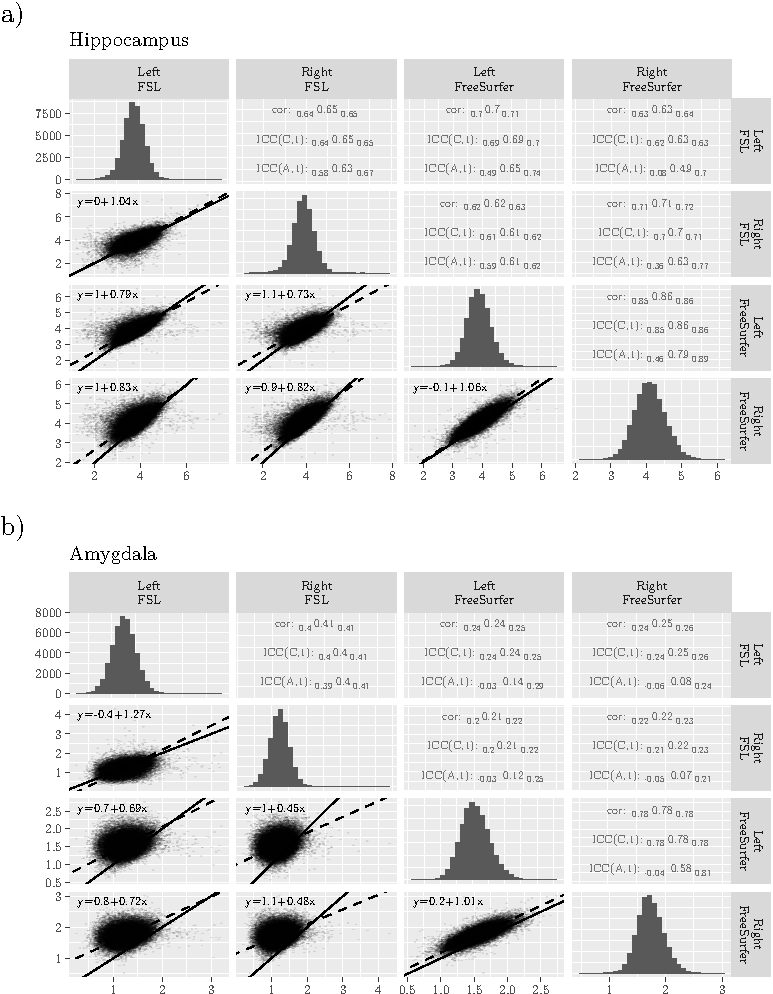
\includegraphics{index_files/figure-pdf/unnamed-chunk-1-1.pdf}

}

\caption{\label{fig-vol-comparison}Comparisons of Subcortical Volumes
Estimated by FSL and FreeSurfer for two example regions a) Hippocampus
and b) Amygdala. For remaining subcortical regions, see
\quartostblref{stbl-iccs}. In the lower triangular panels, the line of
equivalence is marked with a solid line, and the dashed lines show the
result of orthogonal regression. In the upper panel, the uncertainty
estimates span 95\% confidence intervals. The histograms along the
diagonal display volumes in the full sample.}

\end{figure}%

Across all structures, estimated agreement was lower than estimated
consistency (\quartostblref{stbl-iccs}), reflecting differences in the
average volumes estimated by the two methods (\ref{sec-avg-shift}).
However, a constant shift across participants would not affect many
analyses targeted by our primary concern, analyses related to estimated
correlations between regional volumes and some other measure. For that
reason, we focus not on agreement but instead on consistency.

Consistency varies by region (Figure~\ref{fig-vol-comparison},
\quartostblref{stbl-iccs}). To interpret the intraclass correlations,
consider the categories provided by \citet{cicchetti1981}: \textless0.4:
poor, {[}0.4, 0.6): fair, {[}0.6, 0.75): good, {[}0.75, 1): excellent.
Using those categories, the methods exhibit ``good'' to ``excellent''
consistency for most regions. However, the consistency of volumes for
the amygdala is markedly worse than the others, being around only
\textsubscript{0.24}0.24\textsubscript{0.25} and
\textsubscript{0.21}0.22\textsubscript{0.23} for the left and right
hemispheres (ranges of uncertainty span 95\% confidence intervals).
Compare those values to the values for the hippocampus
(Figure~\ref{fig-vol-comparison}), which has good consistency (left:
\textsubscript{0.69}0.69\textsubscript{0.70}, right:
\textsubscript{0.70}0.70\textsubscript{0.71}). For both structures (that
is, the amygdala and hippocampus), consistency across hemispheres as
reported by FreeSurfer is the highest numerically
(Figure~\ref{fig-vol-comparison}). For the amygdala, there is a two-way
interaction between method and hemisphere (FSL - FreeSurfer: 0.22,
\(p<0.001\)), with FreeSurfer reporting that the right amygdala is
larger than the left (left - right: -0.19, \(p<0.001\)) and FSL
reporting that the left is larger than the right (left - right: 0.04,
\(p<0.001\)).

The amygdala has been described as particularly challenging to segment;
one small study (N=23) reports a consistency of 0.6 for volumes
estimated by FSL across repeated scans of the same individual
\citep{morey2010}. Moreover, automated segmentation algorithms can be
affected by experimental factors like site, scanner, participant
positioning, and software version
\citep{hedges2022, du2021, mcguire2017, yang2016, liu2020, mulder_hippocampal_2014, morey2010, perlaki2017},
and differential sensitivity to such factors could impact an intraclass
correlation. In the UKB, several potentially confounding factors were
correlated with estimates of amygdalar volume
(\quartosfigref{sfig-partials-amyg}). However, regressing these factors
from the estimates of volume did not improve the consistency between the
methods (\ref{sec-confounds}).

With poor consistency between measurements of the amygdala, there is
concern that reported relationships involving amygdala volumes may
depend on which method is used for estimating the volume, a choice that
may be considered arbitrary or lab-specific. At least two kinds of
issues could arise. First, lower consistency could make it more likely
that one but not both methods leads to significant correlations. Second,
lower consistency could make it more likely that the two methods produce
significant correlations that go in opposite directions.

\begin{figure}

\centering{

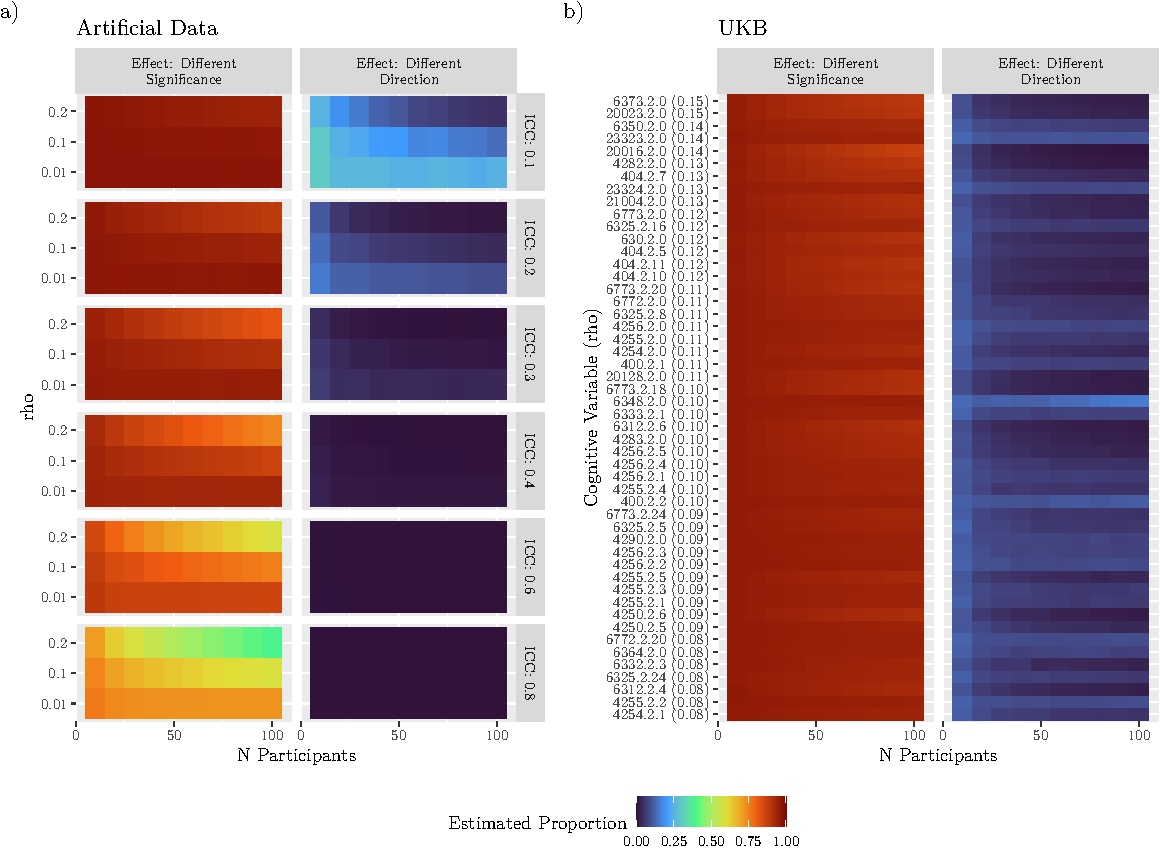
\includegraphics{index_files/figure-pdf/unnamed-chunk-2-1.pdf}

}

\caption{\label{fig-sm-errors}Effects of Low Measurement Consistency. In
the subfigures, the left column or panel shows the proportion of
simulated experiments where the methods produce correlations on opposite
sides of an \(\alpha=0.05\) significance threshold. The right column or
panel shows the proportion of simulated experiments where both measures
are significantly correlated with an outcome but in opposite directions.
Proportions are shown with color \citep{swihart_lasagna_2010}. a)
Simulations with Artificial Data. Rows (rho) indicate pre-specified
product-moment correlation with the outcome variable. ICC: pre-specified
intraclass correlation between measures of volume. b) Simulations with
UKB. Each row corresponds to a non-image derived phenotype from the UKB.
The value in parentheses is the absolute correlation of the variable
with the average volumes of the left amygdala (average across methods).
For a display without color that includes estimates of uncertainty, see
\quartosfigref{sfig-left-right}.}

\end{figure}%

To investigate how often these two issues could occur, we first
simulated experiments with artificial data. In each simulation, datasets
with two noisy estimates of volume and a third, outcome, variable were
generated such that the two volume estimates had a pre-specified
intraclass correlation with each other (in expectation), and the true
volume had a given product-moment correlation with the outcome variable.
The estimated volumes were then tested for a product-moment correlation
with the outcome, and the process was repeated for several intraclass
correlations and sample sizes. In all simulations, the true
product-moment correlation was set to a value that is either typical for
neuroimaging research \citep[0.1,][]{marek_reproducible_2022}, small but
non-zero (0.01), or large (0.2). For additional details on the
simulation methods, see \ref{sec-sim-details}.

With lower consistency, the estimated product-moment correlations were
more often on opposite sides of a significance threshold
(Figure~\ref{fig-sm-errors}\(\~\)a, left column). For example, with
consistency near the value that was estimated for volumes of the
amygdala in the UKB (0.2), a typical effect size (0.1), and experiments
with 50 participants, significance differed in around
\textsubscript{94.9}95.0\textsubscript{95.1} percent of simulations in
which one test was significant (for simulations, estimates indicate
medians and ranges of uncertainty span 95\% equal-tailed intervals, see
\ref{sec-sim-details}). With a sample size of 100, that percentage was
only minimally different (to
\textsubscript{93.7}93.9\%\textsubscript{94.0}). For a discussion on
this insensitivity to sample size, see Section~\ref{sec-min}.

Lower consistency also coincided with a higher proportion of experiments
in which the two methods correlate in opposite directions
(Figure~\ref{fig-sm-errors}\(\~\)a, right column). Considering the
previous example (an intraclass correlation of 0.2, an effect size of
0.1, and 50 participants per experiment), around
\textsubscript{5.13}5.71\textsubscript{6.33} percent of experiments in
which both product-moment correlations were significant resulted in the
correlations having opposite signs. As the intraclass correlation
increased, the rates of this effect decreased rapidly.

To assess how often these two issues could occur in practice, we
repeated the above analyses but with the UKB. From the UKB, we extracted
the ``Cognitive'' variables using the FMRIB UKBiobank Normalisation,
Parsing And Cleaning Kit \citep{mccarthy_funpack_2023}, restricting
analyses to variables with instance 2 and that exhibited one of the
largest (in absolute magnitude) 50 rank correlations (between the
cognitive variables and the average of the two estimates of the volume
of the left amygdala), and further to only those participants that had
values for all 50 of those variables (23486 participants). Each
simulation resulted in a rank correlation between the two volume
estimates for the left amygdala and each of the 50 variables (results
were comparable with the right amygdala). For additional details, see
\ref{sec-sim-details}.

Considering differing significance levels, the rates across experiments
using the UKB resembled the rates from experiments with artificial data.
In simulated experiments with 50 UKB participants in which at least one
correlation was significant, one correlation was not significant in
between \textsubscript{90.7}90.8\textsubscript{91.0} and
\textsubscript{95.1}95.2\textsubscript{95.3} percent of simulations (the
two estimates cover the 50 cognitive variables;
Figure~\ref{fig-sm-errors}\(\~\)b, left panel). Proportions were
generally lower for variables that were more strongly correlated with
the measure of volume (for illustration, compare the variables that are
higher versus lower in the left panel of
Figure~\ref{fig-sm-errors}\(\~\)b).

Considering significant correlations with differing signs, the rates
across experiments with the UKB bracketed the rates with artificial
data. In experiments simulated with 50 UKB participants, the rates
ranged from \textsubscript{1.28}1.45\textsubscript{1.64} to
\textsubscript{7.64}8.32\textsubscript{9.03}. For most variables,
increasing the number of participants decreased the proportion of
experiments in which the two correlations exhibited opposite signs, but
for some the proportion increased. Across the 50 variables, 9 had a
higher proportion at N=100 than N=50, 2 of which had non-overlapping
95\% equal-tailed intervals (6348: duration to complete numeric path;
400: time to complete round of pairs matching game; see also
\quartosfigref{sfig-left-right}).

\section{Discussion}\label{discussion}

We examined the consistency of subcortical volumes within the UK Biobank
\citep{alfaro-almagro_image_2018}, observing that two common methods of
estimating the volume of the amygdala, one from FSL and one from
FreeSurfer, have poor consistency with each other. The main concern in
this report is that consistency this poor can lead to conflicting
results. Two kinds of conflict were explored: the methods producing
correlations that are on opposite sides of significance thresholds, and
the methods producing volumes with significant correlations that have
differing signs. The prevalence of these occurrences was estimated with
artificial data and data from the UKB. Based on the observed rates, we
make the following recommendations.

\subsection{Recommendations}\label{recommendations}

\subsubsection{When testing for new biomarkers, report relationships
with multiple automated methods (e.g., both FSL and
FreeSurfer).}\label{when-testing-for-new-biomarkers-report-relationships-with-multiple-automated-methods-e.g.-both-fsl-and-freesurfer.}

Researchers may have idiosyncratic reasons for selecting a method,
particularly when the choice is viewed as arbitrary. If the choice
between methods is arbitrary, then reporting the outcome across
selections clarifies the fragility or robustness of a result \citep[for
a general discussion, see][]{steegen_increasing_2016}. The choice may
not always be arbitrary, as there are metrics along which and study
populations for which one method may perform better
\citep{zhou_charting_2021, morey2009, huizinga_differences_2021}. Note
that one effect of low consistency could be a downward bias on the
magnitude of estimated correlations
(Section~\ref{sec-measurement-error}), and so there may be advantages to
not only reporting but also combining the estimates across methods when
predicting health-related outcomes (e.g., by averaging, or including
both as independent variables in predictive models). Reporting estimates
from multiple reasonable tools will help move conclusions beyond ``there
exists a correlation with the volume of the amygdala as estimated by
method M (version x)'' to simply ``there exists a correlation with the
volume of the amygdala''.

\subsubsection{When reviewing or conducting meta-analyses of
relationships with amygdala volume, consider the method that was used to
estimate
volume.}\label{when-reviewing-or-conducting-meta-analyses-of-relationships-with-amygdala-volume-consider-the-method-that-was-used-to-estimate-volume.}

As mentioned in the Introduction, the amygdala has received substantial
attention due to being predictive of an array of health-related
outcomes. As presented in this report, the volume that is estimated by
one automated method may only weakly correspond to the volume estimated
by another, and so it may be misleading to conduct a meta-analysis
without accounting for the algorithms used by the individual studies. In
the UKB, there are differences in the strength of the correlations
between the measures of volume and the cognitive variables; in nearly
all of the variables considered in this report, the magnitude of the
correlations involving FreeSurfer's method were numerically larger
(\quartosfigref{sfig-pop-cor}). Larger correlations do not imply higher
veracity, but they further indicate that the methods track aspects of
amygdalar anatomy differently.

\subsubsection{When replicating or extending research on a relationship
that involves the volume of the amygdala, use the method reported in the
original
publications.}\label{when-replicating-or-extending-research-on-a-relationship-that-involves-the-volume-of-the-amygdala-use-the-method-reported-in-the-original-publications.}

This recommendation follows standard practice for a replication study.
We highlight it here in consideration of both extension studies that aim
to apply a biomarker or biosignature that includes amygdala volume (such
as when testing a putative relationship in a new population), and also
in consideration of the ongoing evolution of methods for automatically
estimating subcortical volumes. Although FSL and FreeSurfer are two of
the most popular methods, others exist \citep[e.g.,][]{akhondi-asl2013},
including newer techniques based on deep-learning approaches
\citetext{\citealp[e.g.,][]{billot2023}; \citealp[for review,
see][]{singh2021}}. Newer methods may have better correspondence with
manual segmentation, warranting their use in replication or extension
studies. But as this report shows, two methods can perform well while
exhibiting poor consistency with each other. So when building on prior
findings, it remains important to use the methods of those prior
findings, even when they are superseded.

\section*{Data and Code Availability}\label{data-and-code-availability}
\addcontentsline{toc}{section}{Data and Code Availability}

Imaging data underlying the results presented are available from the UK
Biobank upon successful application
(https://www.ukbiobank.ac.uk/enableyourresearch/apply-for-access). Code
to reproduce analyses is available on GitHub:
https://github.com/psadil/auto-volume-comparisons.

\section*{Author Contributions}\label{author-contributions}
\addcontentsline{toc}{section}{Author Contributions}

\textbf{Patrick Sadil}: Conceptualization, Methodology, Software,
Validation, Formal Analysis, Investigation, Resources, Data Curation,
Writing - Original Draft, Writing - Review \& Editing, Visualization.
\textbf{Martin A. Lindquist}: Conceptualization, Methodology,
Validation, Formal Analysis, Resources, Writing - Original Draft,
Writing - Review \& Editing, Supervision, Project Administration,
Funding Acquisition.

\section*{Declaration of Competing
Interest}\label{declaration-of-competing-interest}
\addcontentsline{toc}{section}{Declaration of Competing Interest}

The authors declare that they have no known competing financial
interests or personal relationships that could have appeared to
influence the work reported in this paper.

\section*{Ethics Statement}\label{ethics-statement}
\addcontentsline{toc}{section}{Ethics Statement}

Informed consent was obtained from all UK Biobank participants. Ethical
procedures are controlled by a dedicated Ethics Advisory Committee
(http://www.ukbiobank.ac.uk/ethics).

\section*{Acknowledgements}\label{acknowledgements}
\addcontentsline{toc}{section}{Acknowledgements}

This work was supported by grant R01MH129397 from the National Institute
of Mental Health. This research has been conducted using data from UK
Biobank, a major biomedical database (Project ID: 33278). We are
grateful to UK Biobank and the UK Biobank participants for making the
resource data possible, and to the data processing team at Oxford
University for sharing the processed data. The UK Biobank imaging
project is funded by the Medical Research Council and the Wellcome
Trust.

\section*{References}\label{references}
\addcontentsline{toc}{section}{References}

\renewcommand{\bibsection}{}
\bibliography{references.bib}

\newpage
\appendix

\section{Supplementary Materials}\label{sec-supplements}

\subsection{Intraclass Correlation}\label{sec-icc-models}

The intraclass correlation was based on a two-way mixed linear model
\citep{mcgraw1996}. In the model, the volume \(x\) for the region of
participant \(i\) as measured by method \(k\) was treated as equal to
the sum of an intercept, \(\nu\), the ``true'' volume, \(\lambda_i\), a
method bias, \(c_k\), and an error term, \(\epsilon_{ik}\)

\[
\begin{aligned}
x_{ik} &= \nu + \lambda_i + c_k + \epsilon_{ik} \\
\sum_k c_k &= 0 \\
\lambda_i &\sim N(0,\sigma_\lambda^2) \\
\epsilon_{ik} &\sim N(0, \sigma_\epsilon^2)
\end{aligned}
\]

Note that the \(c_k\) terms are assumed fixed, with variance given by
\(\sigma_c^2=\sum_k c_k^2/(k-1)\).

An important assumption of this model is that the two methods are
expected to have the same mean-squared error. The model does not include
features that would allow for the errors in the two methods to be
correlated (e.g., participants are not distinguished by characteristics
that coincide with the methods performing better or worse).

The consistency version of the intraclass correlation, \(ICC(C,1)\), and
the absolute agreement, \(ICC(A,1)\) were given as fractions of the
variance components

\[
\begin{aligned}
ICC(C,1) & = \frac{\sigma_\lambda^2}{\sigma_\lambda^2 + \sigma_\epsilon^2} \\
ICC(A,1) & = \frac{\sigma_\lambda^2}{\sigma_\lambda^2 + \sigma_\epsilon^2 + \sigma_c^2}
\end{aligned}
\]

Variance components and associated confidence intervals estimated using
the \texttt{R} package \texttt{irr} \citep{core_r_2023, gamer_irr_2019},
which uses the mean square approach described by \citet{mcgraw1996}.

\subsection{Differences in Average Volumes}\label{sec-avg-shift}

Although we primarily focused on the consistency of the methods, we also
observed shifts in the average volumes reported by the two methods
(\quartosfigref{sfig-biases-perc}). Differences in averages across
methods have been reported previously
\citep{gomez-ramirez2022, perlaki2017, dewey2010, huizinga_differences_2021}.
FSL tends to report volumes that are larger than those from FreeSurfer
for the Accumbens, Amygdala, Hippocampus, and Pallidum, whereas for the
Caudate, Putamen, and Thalamus FSL tends to report values that are
smaller than those from FreeSurfer (all \(p < 0.0001\) for two-sided
t-test). Across structures, the variability in the difference appears to
covary with the average of the two volume estimates, increasing as the
average volume estimate decreases (\quartosfigref{sfig-biases-perc} b).

\begin{sfig}

\centering{

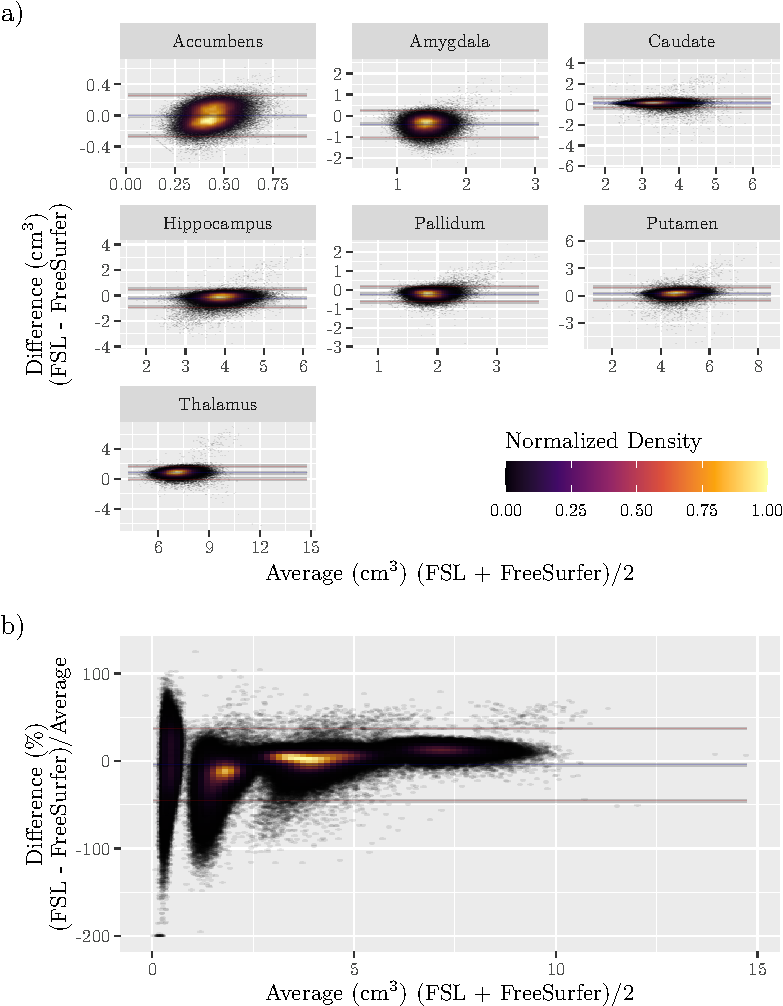
\includegraphics{index_files/figure-pdf/sfig-biases-perc-1.pdf}

}

\caption{\label{sfig-biases-perc}Bland-Altman Plots for Subcortical
Volume. Horizontal lines show average difference and limits of agreement
(1.96 standard deviations), with ribbons marking 95\% confidence
intervals. Panels correspond to subcortical structures. Left and right
structures are plotted together. Shifts in the average estimate
correspond to the central ribbon excluding zero. The color overlay
indicates the degree of overplotting. a) Raw Differences. Note that axes
are across panels independently. b) Differences by Percent Average.}

\end{sfig}%

\FloatBarrier

\subsection{Intraclass Correlations Across All Subcortical
Regions}\label{sec-other-structs}

\begin{stbl}

\centering{

\begin{longtable*}{llcc}
\toprule
Structure & Hemisphere & ICC(C,1) & ICC(A,1) \\ 
\midrule\addlinespace[2.5pt]
Accumbens & Left & $_{0.57}$0.58$_{0.58}$ & $_{ 0.05}$0.44$_{0.65}$ \\ 
Accumbens & Right & $_{0.56}$0.57$_{0.57}$ & $_{-0.03}$0.38$_{0.63}$ \\ 
Amygdala & Left & $_{0.24}$0.24$_{0.25}$ & $_{-0.03}$0.14$_{0.29}$ \\ 
Amygdala & Right & $_{0.21}$0.22$_{0.23}$ & $_{-0.05}$0.07$_{0.21}$ \\ 
Caudate & Left & $_{0.85}$0.85$_{0.86}$ & $_{ 0.75}$0.83$_{0.88}$ \\ 
Caudate & Right & $_{0.86}$0.86$_{0.87}$ & $_{ 0.62}$0.82$_{0.90}$ \\ 
Hippocampus & Left & $_{0.69}$0.69$_{0.70}$ & $_{ 0.49}$0.65$_{0.74}$ \\ 
Hippocampus & Right & $_{0.70}$0.70$_{0.71}$ & $_{ 0.36}$0.63$_{0.77}$ \\ 
Pallidum & Left & $_{0.68}$0.68$_{0.69}$ & $_{-0.09}$0.41$_{0.71}$ \\ 
Pallidum & Right & $_{0.66}$0.67$_{0.67}$ & $_{ 0.04}$0.51$_{0.73}$ \\ 
Putamen & Left & $_{0.79}$0.79$_{0.80}$ & $_{ 0.54}$0.74$_{0.84}$ \\ 
Putamen & Right & $_{0.82}$0.83$_{0.83}$ & $_{ 0.56}$0.77$_{0.87}$ \\ 
Thalamus & Left & $_{0.82}$0.82$_{0.83}$ & $_{-0.08}$0.49$_{0.79}$ \\ 
Thalamus & Right & $_{0.83}$0.83$_{0.83}$ & $_{-0.09}$0.51$_{0.81}$ \\ 
\bottomrule
\end{longtable*}

}

\caption{\label{stbl-iccs}Intraclass Correlation for Subcortical
Structures. Subscripts indicate 95\% confidence intervals.}

\end{stbl}%

\FloatBarrier

\subsection{Intraclass Correlations After Residualizing on Potential
Confounds}\label{sec-confounds}

One possible source of low intraclass correlations could be systematic
inaccuracies with certain kinds of participants. For example, one of the
two methods could tend to underestimate volumes when given brains that
have experienced severe atrophy, which would decrease the agreement of
the methods. To assess this, correlations between the amygdala volumes
and the ``simple'' confounds within the UKB were calculated
\citep{alfaro-almagro2021}.

Several of the correlations appeared to be non-zero
(\quartosfigref{sfig-partials-amyg}). However, regressing these
confounds from the estimated amygdala volumes did not improve the
intraclass correlations (\quartostblref{stbl-iccs-deconfounded}).

\begin{sfig}

\centering{

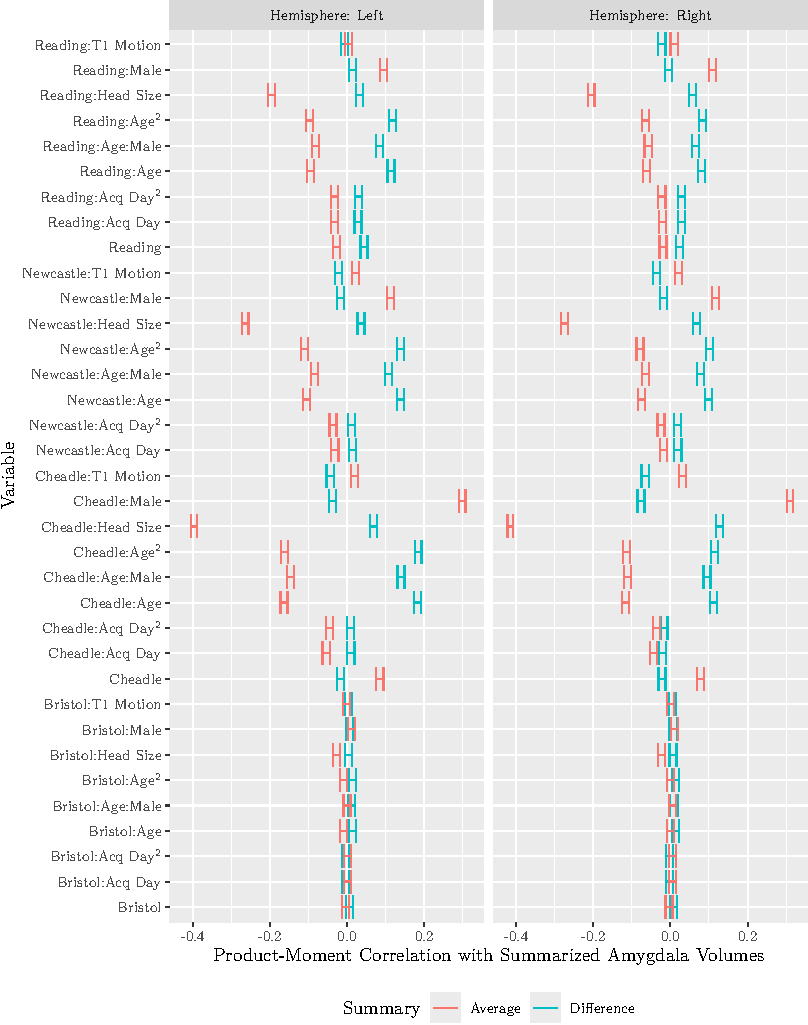
\includegraphics{index_files/figure-pdf/sfig-partials-amyg-1.pdf}

}

\caption{\label{sfig-partials-amyg}Correlation Between Potential
Confounders and Amygdala Volume Measurements. Summary describes how the
the volumes were combined across methods. Summaries were either an
average or a difference (FSL-FreeSurfer). Note that the variable ``Head
Size'' corresponds to a scaling factor, and that larger values imply
smaller brains.}

\end{sfig}%

\begin{stbl}

\centering{

\begin{longtable*}{llcc}
\toprule
Structure & Hemisphere & ICC(C,1) & ICC(A,1) \\ 
\midrule\addlinespace[2.5pt]
Accumbens & Left & $_{0.42}$0.43$_{0.44}$ & $_{ 0.01}$0.30$_{0.51}$ \\ 
Accumbens & Right & $_{0.44}$0.45$_{0.45}$ & $_{-0.05}$0.27$_{0.51}$ \\ 
Amygdala & Left & $_{0.07}$0.08$_{0.09}$ & $_{-0.01}$0.04$_{0.10}$ \\ 
Amygdala & Right & $_{0.04}$0.05$_{0.06}$ & $_{-0.01}$0.01$_{0.04}$ \\ 
Caudate & Left & $_{0.81}$0.81$_{0.81}$ & $_{ 0.68}$0.78$_{0.84}$ \\ 
Caudate & Right & $_{0.82}$0.82$_{0.82}$ & $_{ 0.52}$0.76$_{0.86}$ \\ 
Hippocampus & Left & $_{0.57}$0.58$_{0.59}$ & $_{ 0.36}$0.53$_{0.64}$ \\ 
Hippocampus & Right & $_{0.58}$0.59$_{0.59}$ & $_{ 0.23}$0.50$_{0.66}$ \\ 
Pallidum & Left & $_{0.55}$0.56$_{0.57}$ & $_{-0.09}$0.30$_{0.59}$ \\ 
Pallidum & Right & $_{0.54}$0.54$_{0.55}$ & $_{-0.01}$0.38$_{0.61}$ \\ 
Putamen & Left & $_{0.68}$0.69$_{0.69}$ & $_{ 0.38}$0.62$_{0.75}$ \\ 
Putamen & Right & $_{0.73}$0.74$_{0.74}$ & $_{ 0.41}$0.66$_{0.79}$ \\ 
Thalamus & Left & $_{0.64}$0.65$_{0.65}$ & $_{-0.08}$0.27$_{0.60}$ \\ 
Thalamus & Right & $_{0.64}$0.65$_{0.65}$ & $_{-0.09}$0.28$_{0.60}$ \\ 
\bottomrule
\end{longtable*}

}

\caption{\label{stbl-iccs-deconfounded}Intraclass Correlation After
Deconfounding. Prior to calculating consistency, volumes were
deconfounded by a version of the ``simple'' parameter set described by
\citet{alfaro-almagro2021}. For the list of variables, see
\quartosfigref{sfig-partials-amyg}. Subscripts indicate 95\% confidence
intervals.}

\end{stbl}%

\FloatBarrier

\subsubsection{Adjusting for ICV}\label{sec-adjust-icv}

When reporting differences in volume between groups, it is common to
adjust for either head size or cerebral volume
\citep{barnes_head_2010, mathalon_correction_1993, voevodskaya_effects_2014}.
Adjusting by intracranial volume as estimated by FreeSurfer did not
improve the intraclass correlations (\quartostblref{stbl-adjust}).

\begin{stbl}

\centering{

\begin{longtable*}{llcc}
\toprule
Structure & Hemisphere & ICC(C,1) & ICC(A,1) \\ 
\midrule\addlinespace[2.5pt]
Accumbens & Left & $_{0.88}$0.88$_{0.88}$ & $_{ 0.40}$0.81$_{0.91}$ \\ 
Accumbens & Right & $_{0.90}$0.90$_{0.90}$ & $_{ 0.23}$0.81$_{0.92}$ \\ 
Amygdala & Left & $_{0.27}$0.28$_{0.29}$ & $_{-0.03}$0.17$_{0.34}$ \\ 
Amygdala & Right & $_{0.20}$0.21$_{0.22}$ & $_{-0.05}$0.07$_{0.20}$ \\ 
Caudate & Left & $_{0.79}$0.80$_{0.80}$ & $_{ 0.67}$0.77$_{0.83}$ \\ 
Caudate & Right & $_{0.81}$0.81$_{0.81}$ & $_{ 0.52}$0.75$_{0.85}$ \\ 
Hippocampus & Left & $_{0.63}$0.63$_{0.64}$ & $_{ 0.42}$0.58$_{0.69}$ \\ 
Hippocampus & Right & $_{0.63}$0.64$_{0.64}$ & $_{ 0.28}$0.55$_{0.71}$ \\ 
Pallidum & Left & $_{0.63}$0.63$_{0.64}$ & $_{-0.09}$0.36$_{0.66}$ \\ 
Pallidum & Right & $_{0.60}$0.61$_{0.61}$ & $_{ 0.02}$0.45$_{0.68}$ \\ 
Putamen & Left & $_{0.72}$0.72$_{0.72}$ & $_{ 0.44}$0.66$_{0.78}$ \\ 
Putamen & Right & $_{0.76}$0.76$_{0.76}$ & $_{ 0.46}$0.70$_{0.81}$ \\ 
Thalamus & Left & $_{0.75}$0.75$_{0.76}$ & $_{-0.09}$0.39$_{0.72}$ \\ 
Thalamus & Right & $_{0.75}$0.76$_{0.76}$ & $_{-0.09}$0.40$_{0.73}$ \\ 
\bottomrule
\end{longtable*}

}

\caption{\label{stbl-adjust}Consistency of Volumes when Adjusting by
Intracranial Volume. Adjustments were done by residualizing with respect
to ICV. Subscripts indicate 95\% confidence intervals.}

\end{stbl}%

\FloatBarrier

\subsection{Simulated Experiments}\label{sec-sim-details}

To simulate hypothetical data, the models described in the previous
sections were used. Sample sizes were set between 10 to 100 in steps of
10. At each combination of parameters, experiments were repeated
1,000,000 times. Simulated experiments with the UKB data were performed
analogously to those with hypothetical data (UKB samples were taken with
replacement).

In all simulations with artificial data, several parameters described in
Section~\ref{sec-icc-models} would not influence results after setting
an intraclass and interclass correlation and so were set to arbitrary
values: \(\nu=0\), \(\sigma_\delta=1\), and \(\sigma_c=0\). The
remaining parameter \(\sigma_\lambda\) was set to a value that was
estimated from the full UKB with a linear mixed-effects model that was
estimated by restricted maximum likelihood as implemented by
\texttt{lme4} \citep{bates_fitting_2015}: 0.019.

Across repetitions, the rates of each effect were estimated by analytic
Bayesian methods (binomial likelihood with Beta prior whose shape
parameters were set to 1/2). For the effect of ``Different
Significance'', the posterior was based on the number of simulations in
which one correlation exhibited a \(p\)-value less than 0.05 and the
other was above 0.05 (successes among relevant simulations) and the
number of simulations in which at least one \(p\)-value was below 0.05
(total relevant simulations). The effect of ``Different Direction'' was
calculated similarly, but used simulations in which both correlations
had opposite magnitudes out of those in which both were significant. In
the main text, ranges of uncertainty refer to 95\% equal-tailed
intervals and proportions refer to posterior medians.

The 95\% equal-tailed interval of the posteriors for the simulations are
shown in \quartosfigref{sfig-left-right}.

\begin{sfig}

\centering{

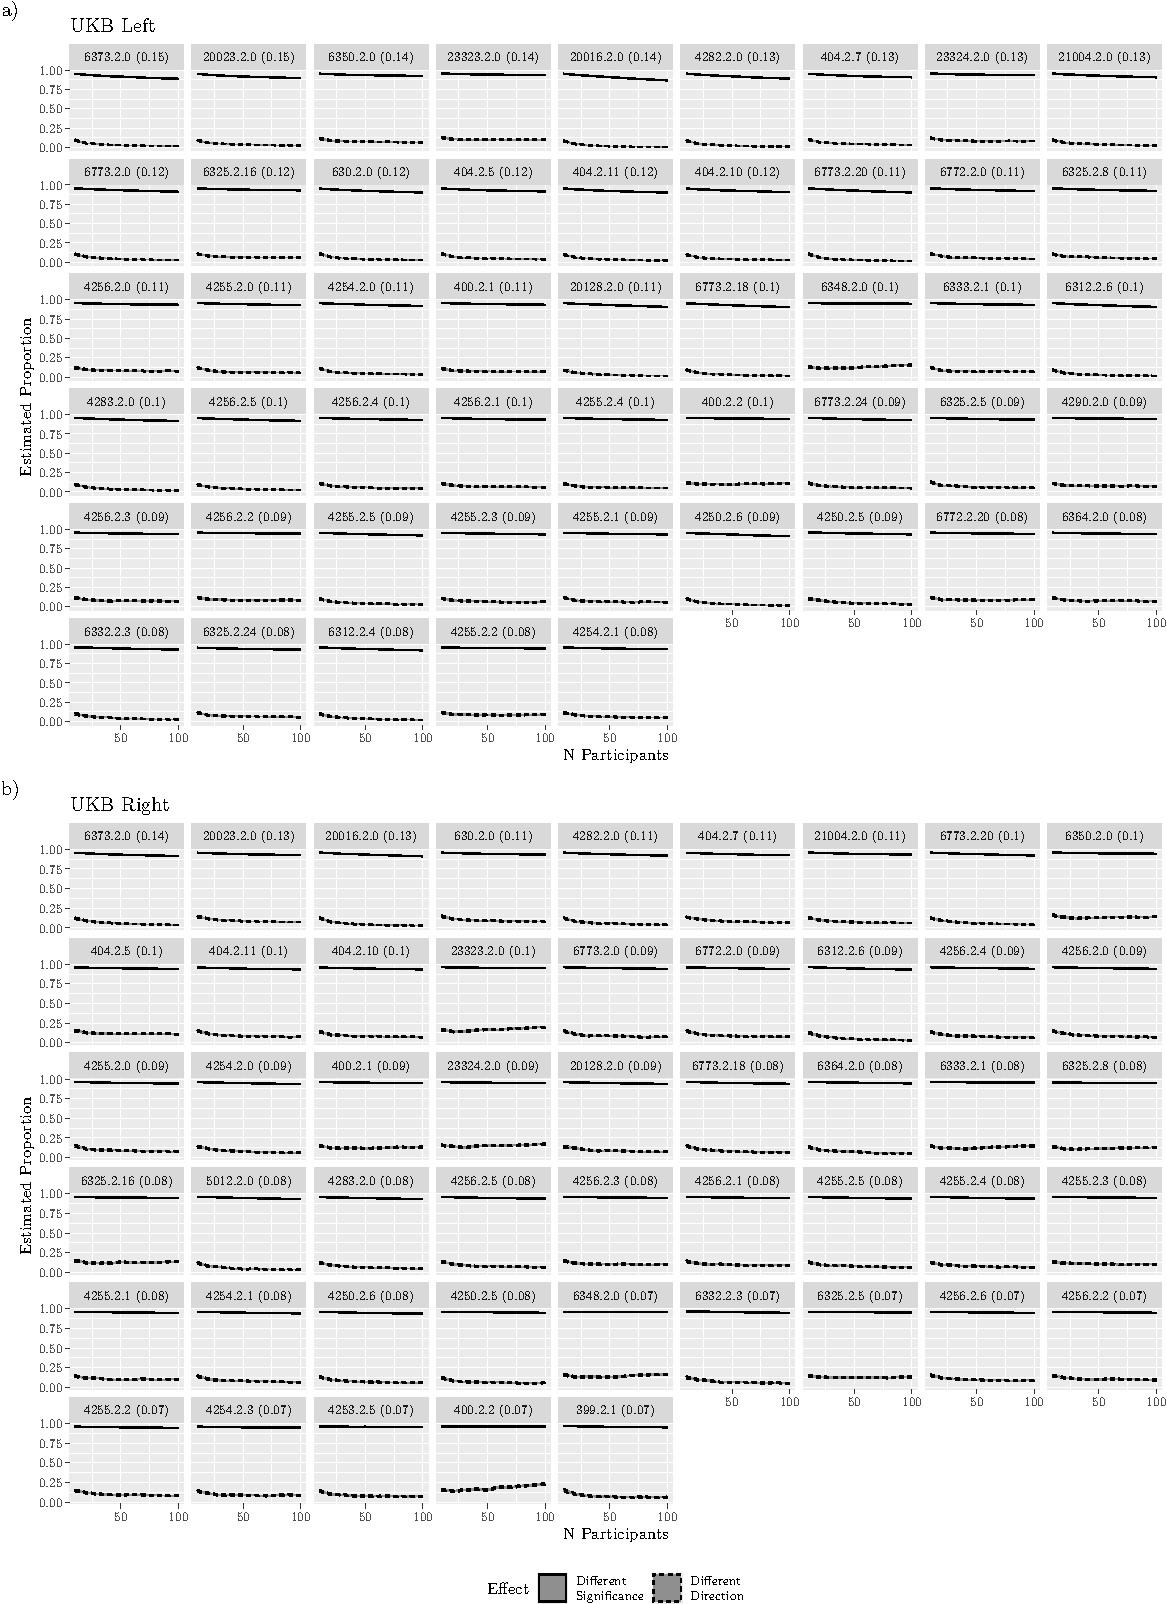
\includegraphics{index_files/figure-pdf/sfig-left-right-1.pdf}

}

\caption{\label{sfig-left-right}Effects of Low Measurement Consistency
on the UKB in Left and Right Hemispheres. Ribbons span 95\% equal-tailed
interval estimated from simulated experiments. See also
Figure~\ref{fig-sm-errors}, where the medians are represented with
color.}

\end{sfig}%

\FloatBarrier

\subsection{Differing Significance Minimally Affected by Increasing
Sample Sizes When ICC is Low}\label{sec-min}

As described in the main text, when intraclass correlations were low,
increasing the sample size affected the rates of differing significance
only minimally Figure~\ref{fig-sm-errors}. This lack of influence can be
understood by inspecting the distribution of simulated correlations
\quartosfigref{sfig-why-flat}. When the intraclass correlation is low
\quartosfigref{sfig-why-flat}, the significance of one correlation is
nearly uninformative about the significance of the other (that is, the
distributions of the two correlations are nearly circular). Moreover,
the power to detect small correlations with even 100 participants is
low, and so the power for two tests is very low. But when the intraclass
correlation is higher \quartosfigref{sfig-why-flat}, the two
correlations cluster, which improves the power of a second test
conditioning on one test being significant.

\begin{sfig}

\centering{

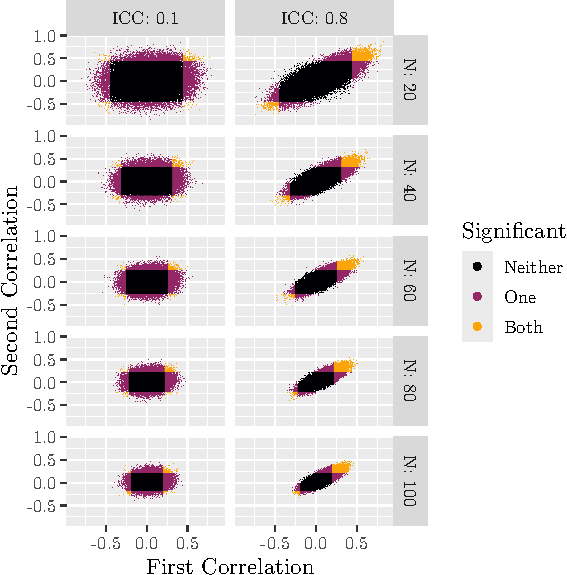
\includegraphics{index_files/figure-pdf/unnamed-chunk-3-1.pdf}

}

\caption{\label{sfig-why-flat}Correlations from Simulations with
Artificial Data. Points correspond to simulations and are colored based
on statistical significance. The figure shows only a subset of the
simulated sample sizes (rows), only the smallest and largest intraclass
correlations (columns), and only simulations in which the true effect
size (correlation) was 0.1.}

\end{sfig}%

\FloatBarrier

\subsection{Measurement Error and Reduced Correlation
Magnitude}\label{sec-measurement-error}

Using the model from \ref{sec-icc-models}, we can build a measurement
noise model \citep[e.g.,][]{frost_correcting_2000}. Call the final
target for which we hope to find a relationship with the volume \(y\).
The relationship between that value and the volume was given by an
ordinary linear regression with error \(\delta\).

\[
\begin{aligned}
y_i & = \beta_0 + \beta_1\lambda_i + \delta_i \\
\delta_i & \sim N(0, \sigma_\delta^2) \\
\end{aligned}
\]

But since we do not know \(\lambda\), the volumes estimated by the tools
are used instead, changing the regression coefficient as follows

\[
y_i = \beta_0 + \tilde{\beta_1}x_i + \delta_i \\
\]

Dilution occurs because the coefficient \(\tilde{\beta_1}\) estimated in
this model tends to be closer to zero, decreased by a factor related to
the intraclass correlation \citep{frost_correcting_2000}.

\[
\tilde{\beta_1} = \beta_1\frac{\sigma_\lambda^2}{\sigma_\lambda^2 + \sigma_\epsilon^2}
\]

Correspondingly, the desired correlation, \(\rho=cor(y,\lambda)\), will
also be biased.

\[
\begin{aligned}
\beta_1 & = \rho\frac{\sigma_\delta}{\sigma_\lambda} \\
\tilde{\beta_1} & = \tilde{\rho}\frac{\sigma_\delta}{sd(x)} \\ 
& =  \tilde{\rho} \frac{\sigma_\delta}{\sqrt{\sigma_\epsilon^2 + \sigma_\lambda^2}} \\
&  \implies \\
\rho \frac{\sigma_\delta}{\sigma_\lambda} &  = \tilde{\rho}\frac{\sigma_\delta}{\sqrt{\sigma_\epsilon^2+\sigma_\lambda^2}} \frac{\sigma_\lambda^2 + \sigma_\epsilon^2}{\sigma_\lambda^2} \\
&  \implies \\
\rho & = \tilde{\rho} \frac{\sqrt{\sigma_\epsilon^2+\sigma_\lambda^2}}{\sigma_\lambda }
\end{aligned}
\]

\FloatBarrier

\subsection{Correlations Between Volumes of the Amygdala and Cognitive
Variables}\label{correlations-between-volumes-of-the-amygdala-and-cognitive-variables}

As described in the main text, a set of 50 ``cognitive'' variables from
the UKB was selected for each hemisphere. Selection was based on the
rank correlation between the variable and the average (across methods)
amygdalar volume. The correlations between those variables and the
original volume estimates are shown in \quartosfigref{sfig-pop-cor}. For
both hemispheres, the magnitude of the correlations with the volumes as
reported by FreeSurfer tended to be higher than those reported by FSL.

\begin{sfig}

\centering{

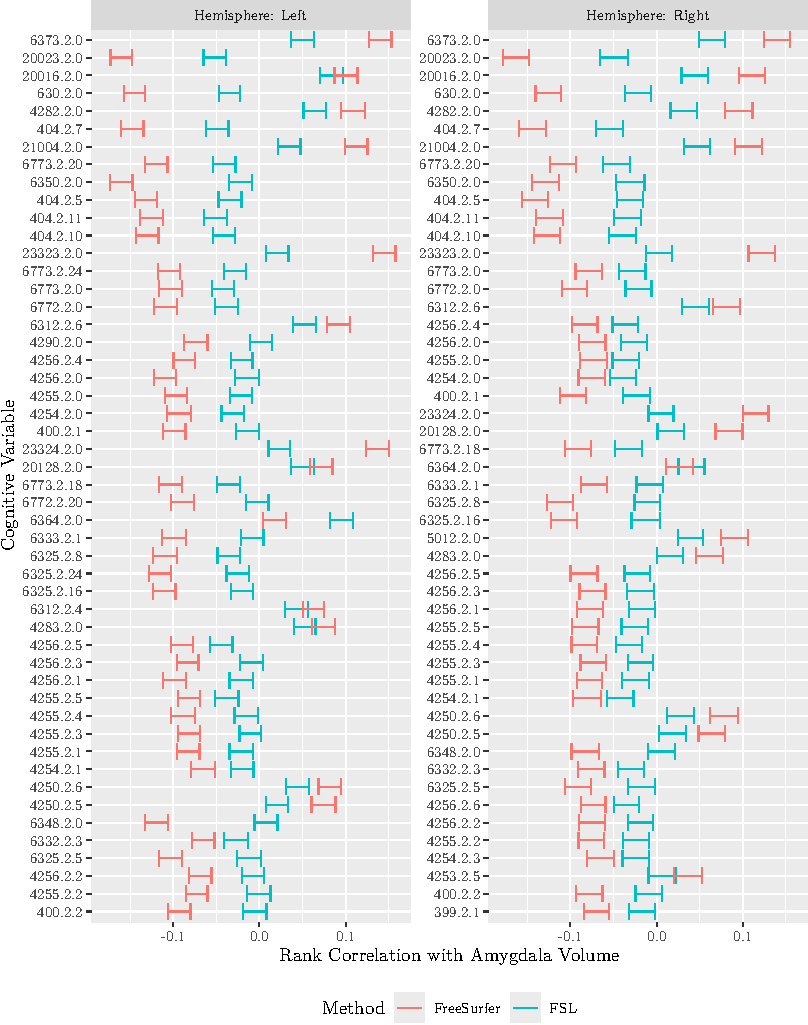
\includegraphics{index_files/figure-pdf/sfig-pop-cor-1.pdf}

}

\caption{\label{sfig-pop-cor}Correlations Between Cognitive Factors and
Estimated Volumes of the Left and Right Amygdala. Variables are ordered
by decreasing rank correlation using average of left hemisphere volume
estimates. Note that variables were selected based on the magnitude of
their correlation with amygdalar volumes, which differed across
hemispheres, and so the variables in left and right panels differ. Error
bars span 95\% confidence intervals (bootstrapped with 1000 samples).}

\end{sfig}%




\end{document}
